% --- IMPORTS ---
\documentclass[leqno]{article}
\usepackage{graphicx}
\usepackage{dsfont}
\usepackage{mathtools}
\usepackage{amssymb}
\usepackage{amsmath}
\usepackage{amsthm}
\usepackage{float}
\usepackage{ragged2e}
\usepackage{tensor}
\usepackage{fancyhdr}
\usepackage{empheq}
\usepackage[most]{tcolorbox}
\usepackage{enumitem}
\usepackage{dirtytalk}
\usepackage{marginnote}
\usepackage{microtype}
\usepackage[
  a4paper,
  left=0.8in,
  right=1in,
  top=1in,
  bottom=0.5in,
  headheight=14pt,
  headsep=0.4in
]{geometry}
\setlength{\parindent}{0cm}
% --- TikZ Packages ---
\usepackage{pgfplots}
\pgfplotsset{compat=1.18}
\usepgfplotslibrary{fillbetween, polar}
\usetikzlibrary{calc, positioning}
\usetikzlibrary{angles, quotes}
\usetikzlibrary{arrows.meta}
\usetikzlibrary{decorations.pathreplacing, decorations.markings}
\usetikzlibrary{patterns}
\usetikzlibrary{intersections}
% --- URL Packages ---
\usepackage[colorlinks=true,linkcolor=red,citecolor=magenta,urlcolor=black]{hyperref}%
\urlstyle{same}
% --- END OF IMPORTS ---

% --- CUSTOM COMMANDS ---
\RenewDocumentCommand{\marks}{o m}{%
  \IfValueTF{#1}%
    {\marginnote{\raggedright\textbf{[#2]}}[#1]}%
    {\marginnote{\raggedright\textbf{[#2]}}}%
}
\newcommand{\vspacerule}[2]{%
  \par\vspace*{#1}%
  \noindent\hrulefill\par
  \vspace*{#2}%
}
\definecolor{scarlet}{RGB}{205, 40, 75}
\newcommand{\questionitem}{%
  \item\phantomsection
  \addcontentsline{toc}{section}{Question \number\value{enumi}}%
}
\renewcommand{\contentsname}{Questions}
\newcommand{\timingbox}[4]{%
  \vspace*{20pt}
  \noindent\begin{tcolorbox}[
    enhanced, sharp corners,
    width=0.8\textwidth,
    colback=white, colframe=white, boxrule=0pt,
    borderline west={3pt}{0pt}{scarlet},
    left=20pt, right=20pt, top=12pt, bottom=12pt,
    before skip=0pt, after skip=0pt
  ]
  {\LARGE\bfseries #1}\\[8pt]
  {\normalsize Total Marks: #2 }\\[6pt]
  {\normalsize  #3\\[6pt]
  Complete in \textbf{#4}}
  \end{tcolorbox}
  \vspace*{20pt}%
}
% --- END OF CUSTOM COMMANDS ---

% --- HEADER CONFIG ---
\pagestyle{fancy}
\fancyhead{}
\fancyfoot{}
\renewcommand{\headrulewidth}{0.9pt}
\lhead{\textit{Solutions} - Work-Energy Principle}
\chead{}
\rhead{\href{https://danieljsmith.org}{danieljsmith.org}}
% --- END OF HEADER CONFIG ---

\begin{document}
\vspace*{20pt}
\tableofcontents
\newpage
\begin{enumerate}[
  label=\textbf{\arabic*.},
  leftmargin=*,
  topsep=0pt,
  partopsep=0pt,
  parsep=0pt
]

% ---- Question 1 ----
\questionitem
% [Source: _QBT___Solns__Work_Energy_Principle, Q1]

\begin{figure}[H]
    \centering
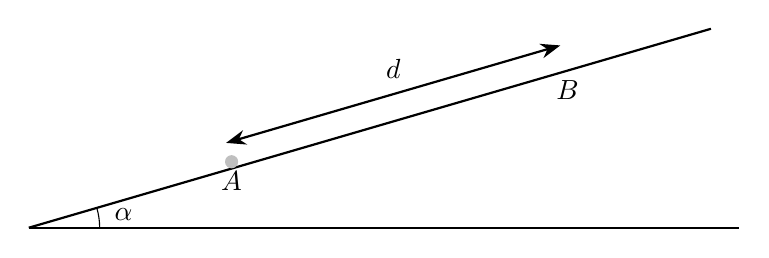
\begin{tikzpicture}[scale=0.95]
\def\run{24}
\def\rise{7}
\def\scaleFactor{0.38}
\def\dimOffset{0.35}
\def\particleRadius{2.5pt}
\pgfmathsetmacro{\ang}{atan(\rise/\run)}
\pgfmathsetmacro{\slopeLen}{\scaleFactor*sqrt(\run*\run+\rise*\rise)}

\coordinate (base) at (0,0);
\coordinate (top) at (\ang:\slopeLen);
\coordinate (Aplane) at ($(base)!0.30!(top)$);
\coordinate (B) at ($(base)!0.79!(top)$);
\coordinate (A) at ($(Aplane)+({90+\ang}:\particleRadius)$);
\coordinate (horiz) at (\slopeLen,0);
\coordinate (dA) at ($(Aplane)+({90+\ang}:\dimOffset)$);
\coordinate (dB) at ($(B)+({90+\ang}:\dimOffset)$);

\draw[thick, black] (base) -- (top);
\draw[thick, black] (base) -- (horiz);
\fill[gray!50, yshift=5pt] (A) circle (\particleRadius);

\node[below] at (A) {$A$};
\node[below] at (B) {$B$};
\draw[{Stealth[length=2.5mm]}-{Stealth[length=2.5mm]}, thick, black]
  (dA) -- node[midway, above=2pt] {$d$} (dB);

\pic["$\alpha$", draw, angle radius=9mm, angle eccentricity=1.35] {angle=horiz--base--top};
\end{tikzpicture}
\end{figure}


A particle of mass $m$ is at a point $A$ on a rough plane. \\

The plane is inclined at an angle $\alpha$ to the horizontal, where $\sin\alpha=\dfrac{7}{25}$. \\

The coefficient of friction between the particle and the plane is $\dfrac{1}{3}$. \\

The points $A$ and $B$ lie on a line of greatest slope of the plane, with $B$ above $A$, and $AB=d$, as shown in the diagram. \\

\begin{enumerate}[label=\textbf{(\alph*)}]
  \item Show that the work done against friction as the particle moves from $A$ to $B$ is
  \[
  \dfrac{8}{25}mgd
  \]
  \marks[-20pt]{3}
  \item The particle is projected up the line of greatest slope from $A$ towards $B$ with speed $\sqrt{gd}$. \\
  Use the work-energy principle to determine whether the particle reaches $B$. If it does not, find how far it travels from $A$ before coming instantaneously to rest. \marks{4} \\
\end{enumerate}

\vspace*{10pt}

\begin{tcolorbox}[colback=white, colframe=scarlet, title={\textbf{Solution}}, breakable, grow to left by=6mm, grow to right by=10mm]
\begin{enumerate}[label=\textbf{(\alph*)}]
  \item Since \(\sin\alpha=\dfrac{7}{25}\), we have
\[
\cos\alpha=\frac{24}{25}
\]

The normal reaction is
\[
R=mg\cos\alpha=mg\cdot \frac{24}{25}=\frac{24}{25}mg
\]

So the friction force is
\[
F=\mu R=\frac13\cdot \frac{24}{25}mg=\frac{8}{25}mg
\]

Hence the work done against friction in moving a distance \(d\) up the plane is
\[
W=Fd=\frac{8}{25}mg\times d=\frac{8}{25}mgd
\]

So the work done against friction is \(\dfrac{8}{25}mgd\).

  \item Let the gravitational potential energy at \(A\) be zero.

First check whether the particle can reach \(B\).  
Using the work-energy principle,
\[
\text{KE}_A+\text{GPE}_A+\sum W=\text{KE}_B+\text{GPE}_B
\]

If the particle reaches \(B\) with speed \(v\), then
\[
\text{KE}_A=\frac12 m(\sqrt{gd})^2=\frac12 mgd
\]
\[
\text{GPE}_B=mg(d\sin\alpha)=mgd\cdot \frac{7}{25}=\frac{7}{25}mgd
\]
and the work done by friction is negative:
\[
\sum W=-\frac{8}{25}mgd
\]

So
\begin{align*}
\frac12 mgd+0-\frac{8}{25}mgd&=\frac12 mv^2+\frac{7}{25}mgd \\
\frac12 mv^2&=\frac12 mgd-\frac{8}{25}mgd-\frac{7}{25}mgd \\
&=\left(\frac12-\frac{15}{25}\right)mgd \\
&=-\frac{1}{10}mgd
\end{align*}

This is impossible, since kinetic energy cannot be negative.

Therefore the particle does not reach \(B\).

Now let the distance travelled from \(A\) before coming instantaneously to rest be \(s\).

Again using
\[
\text{KE}_A+\text{GPE}_A+\sum W=\text{KE}_C+\text{GPE}_C
\]
where \(C\) is the point where it stops:

\[
\text{KE}_A=\frac12 mgd,\qquad \text{KE}_C=0
\]
\[
\text{GPE}_C=mg(s\sin\alpha)=mg s\cdot \frac{7}{25}=\frac{7}{25}mgs
\]
\[
\sum W=-\frac{8}{25}mgs
\]

Hence
\begin{align*}
\frac12 mgd+0-\frac{8}{25}mgs&=0+\frac{7}{25}mgs \\
\frac12 mgd&=\frac{15}{25}mgs \\
\frac12 mgd&=\frac35 mgs
\end{align*}

So
\[
s=\frac{\frac12}{\frac35}d=\frac{5d}{6}
\]

Hence the particle does not reach \(B\), and it travels \(\dfrac{5d}{6}\) from \(A\) before coming to rest.
\end{enumerate}
\end{tcolorbox}


\newpage

% ---- Question 2 ----
\questionitem
% [Source: _QBT___Solns__Work_Energy_Principle, Q2]

A plane is inclined to the horizontal at an angle $\alpha$, where $\tan\alpha=\dfrac{5}{12}$. \\

A point $B$ lies on the plane such that $AB=39\text{ m}$. \\

A particle $P$ is projected with speed $21\text{ m s}^{-1}$ from $A$, up a line of greatest slope of the plane. \\

In an initial model, the plane is modelled as being smooth and air resistance is modelled as being negligible. \\

Using this model and the principle of conservation of mechanical energy, \\

\begin{enumerate}[label=\textbf{(\alph*)}]
  \item find the speed of $P$ when it reaches $B$. \marks{4} \\
\end{enumerate}

In a refined model, the plane is now modelled as being rough, with the coefficient of friction between $P$ and the plane being $\dfrac{1}{3}$. \\

Air resistance is still modelled as being negligible. \\

Using this refined model and the work-energy principle, \\

\begin{enumerate}[label=\textbf{(\alph*)}, resume]
  \item determine whether $P$ reaches $B$. If it does not, find the distance travelled by $P$ up the plane from $A$ before it comes instantaneously to rest. \marks{8} \\
\end{enumerate}

\vspace*{10pt}

\begin{tcolorbox}[colback=white, colframe=scarlet, title={\textbf{Solution}}, breakable, grow to left by=6mm, grow to right by=10mm]
\begin{enumerate}[label=\textbf{(\alph*)}]
  \item Since $\tan\alpha=\dfrac{5}{12}$, we use the $5$-$12$-$13$ triangle, so
  \[
  \sin\alpha=\frac{5}{13}
  \]

  The vertical height gained from $A$ to $B$ is
  \[
  39\sin\alpha=39\cdot\frac{5}{13}=15\text{ m}
  \]

  Taking gravitational potential energy to be $0$ at $A$, and using conservation of mechanical energy,
  \[
  \text{KE at }A+\text{GPE at }A=\text{KE at }B+\text{GPE at }B
  \]
  so
  \[
  \frac12 m(21)^2+0=\frac12 mv^2+mg(15)
  \]

  With $g=9.8$,
  \begin{align*}
  \frac12 m(441) &= \frac12 mv^2 + 15mg \\
  220.5m &= \frac12 mv^2 + 147m \\
  \frac12 mv^2 &= 73.5m \\
  v^2 &= 147
  \end{align*}

  Hence
  \[
  v=\sqrt{147}=7\sqrt{3}\text{ m s}^{-1}
  \]

  So the speed of $P$ at $B$ is $7\sqrt{3}\text{ m s}^{-1}\approx 12.1\text{ m s}^{-1}$

  \item Again, from $\tan\alpha=\dfrac{5}{12}$,
  \[
  \sin\alpha=\frac{5}{13}, \qquad \cos\alpha=\frac{12}{13}
  \]

  The normal reaction is
  \[
  R=mg\cos\alpha=mg\cdot\frac{12}{13}=\frac{12mg}{13}
  \]

  Since the coefficient of friction is $\dfrac13$, the frictional force has magnitude
  \[
  F=\mu R=\frac13\cdot\frac{12mg}{13}=\frac{4mg}{13}
  \]

  To test whether $P$ reaches $B$, use the work-energy principle in the form
  \[
  \text{KE}_0+\text{GPE}_0+\sum W=\text{KE}_1+\text{GPE}_1
  \]

  Between $A$ and $B$, the only non-conservative work is the work done by friction, which is
  \[
  -Fs=-\frac{4mg}{13}\cdot 39=-12mg
  \]

  Also, the gain in height is still $15$ m, so the gain in GPE is $15mg$.

  Therefore
  \[
  \frac12 m(21)^2+0-12mg=\frac12 mv^2+15mg
  \]

  Substituting $g=9.8$,
  \begin{align*}
  220.5m-117.6m &= \frac12 mv^2+147m \\
  102.9m &= \frac12 mv^2+147m \\
  \frac12 mv^2 &= -44.1m
  \end{align*}

  This is impossible, since kinetic energy cannot be negative. Therefore $P$ does not reach $B$.

  Now let the distance travelled up the plane before coming to rest be $s$ m.

  At the turning point, the speed is $0$, so using
  \[
  \text{KE}_0+\text{GPE}_0+\sum W=\text{KE}_1+\text{GPE}_1
  \]
  gives
  \[
  \frac12 m(21)^2+0-\frac{4mg}{13}s=0+mg(s\sin\alpha)
  \]

  Since $\sin\alpha=\dfrac{5}{13}$,
  \[
  220.5m-\frac{4mg}{13}s=\frac{5mg}{13}s
  \]

  So
  \begin{align*}
  220.5m &= \frac{9mg}{13}s \\
  220.5 &= \frac{9\times 9.8}{13}s \\
  s &= \frac{220.5\times 13}{9\times 9.8} \\
  s &= 32.5
  \end{align*}

  Since $32.5<39$, the particle does not reach $B$.

  Therefore, $P$ does not reach $B$, and it travels $32.5\text{ m}$ up the plane before coming instantaneously to rest.
\end{enumerate}
\end{tcolorbox}


\newpage

% ---- Question 3 ----
\questionitem
% [Source: _QBT___Solns__Work_Energy_Principle, Q3]

A sledge of mass $40\,\mathrm{kg}$ is pulled up a rough slope inclined at $10^\circ$ to the horizontal. \\

The coefficient of friction between the sledge and the slope is $0.25$. \\

The sledge is at rest when a rope starts to pull it. \\

The tension in the rope is $220\,\mathrm{N}$ and the rope makes an angle of $15^\circ$ above the slope. \\

After the sledge has moved $5$ metres up the slope, the rope breaks. \\

\begin{enumerate}[label=\textbf{(\alph*)}]
  \item Use an energy method to find the maximum speed of the sledge. \marks{4} \\
  \item Use an energy method to find the total distance the sledge moves up the slope before coming to rest. \marks{2} \\
  \item A student claims that in reality the sledge is unlikely to move more than $6.8$ metres up the slope in total. Comment on the validity of this claim. \marks{2} \\
\end{enumerate}

\vspace*{10pt}

\begin{tcolorbox}[colback=white, colframe=scarlet, title={\textbf{Solution}}, breakable, grow to left by=6mm, grow to right by=10mm]
\begin{enumerate}[label=\textbf{(\alph*)}]
  \item While the rope is pulling, first find the normal reaction.

  Resolving perpendicular to the slope,
  \[
  R + 220\sin 15^\circ = 40g\cos 10^\circ
  \]
  so
  \[
  R = 40g\cos 10^\circ - 220\sin 15^\circ
  \]

  With \(g=9.8\),
  \[
  R = 40(9.8)\cos 10^\circ - 220\sin 15^\circ \approx 329.1\ \mathrm{N}
  \]

  Hence the friction force is
  \[
  F=\mu R=0.25R
  \]

  Now apply the Work-Energy principle over the first \(5\) m:

  \[
  \text{KE}_0+\text{GPE}_0+\sum W=\text{KE}_1+\text{GPE}_1
  \]

  The sledge starts from rest, so \(\text{KE}_0=0\).  
  Take the initial position as zero GPE, so \(\text{GPE}_0=0\).

  The work done by the tension is
  \[
  W_T=220\times 5\cos 15^\circ
  \]

  The work done against friction is
  \[
  W_f=-0.25R\times 5
  \]

  The increase in GPE is
  \[
  40g\times 5\sin 10^\circ
  \]

  So
  \begin{align*}
  0+0+220(5)\cos 15^\circ -0.25R(5)
  &= \frac12(40)v^2 + 40g(5)\sin 10^\circ
  \end{align*}

  Substituting \(R=40g\cos 10^\circ-220\sin 15^\circ\),
  \begin{align*}
  220(5)\cos 15^\circ -0.25\bigl(40g\cos 10^\circ-220\sin 15^\circ\bigr)(5)
  &= \frac12(40)v^2 + 40g(5)\sin 10^\circ
  \end{align*}

  Rearranging,
  \begin{align*}
  \frac12(40)v^2
  &=220(5)\cos 15^\circ-40g(5)\sin 10^\circ-0.25\bigl(40g\cos 10^\circ-220\sin 15^\circ\bigr)(5) \\
  &\approx 310.8
  \end{align*}

  Hence
  \[
  20v^2=310.8
  \]
  \[
  v^2=15.54
  \]
  \[
  v\approx 3.94\ \mathrm{m\,s^{-1}}
  \]

  While the rope is intact, all forces are constant, so the acceleration is constant. The resultant force is up the slope, so the speed increases until the rope breaks. Therefore this is the maximum speed.

  The maximum speed is \(3.94\ \mathrm{m\,s^{-1}}\).

  \item After the rope breaks, the sledge still moves up the slope, then comes to rest.

  Now the normal reaction is simply
  \[
  R=40g\cos 10^\circ
  \]
  so the friction force is
  \[
  0.25\times 40g\cos 10^\circ
  \]

  Let the further distance travelled be \(s\) m.

  Using the Work-Energy principle from the instant the rope breaks until the sledge comes to rest,
  \[
  \text{KE}_0+\text{GPE}_0+\sum W=\text{KE}_1+\text{GPE}_1
  \]

  From part (a), the kinetic energy at the break is \(310.8\) J. Also \(\text{KE}_1=0\).

  Therefore
  \begin{align*}
  310.8 - 0.25(40g\cos 10^\circ)s
  &= 40g(\sin 10^\circ)s
  \end{align*}

  So
  \[
  310.8 = 40g(\sin 10^\circ + 0.25\cos 10^\circ)s
  \]

  Hence
  \[
  s=\frac{310.8}{40(9.8)(\sin 10^\circ+0.25\cos 10^\circ)} \approx 1.89
  \]

  So the total distance moved up the slope is
  \[
  5+1.89=6.89\ \mathrm{m}
  \]

  The total distance is \(6.89\ \mathrm{m}\).

  \item The model gives a total distance of \(6.89\ \mathrm{m}\), so according to the model the sledge would move slightly more than \(6.8\ \mathrm{m}\).

  So the claim is not proved by the model. However, \(6.8\) m is only \(0.09\) m less than the model value, and in reality quantities such as friction and tension may vary, so a slightly smaller distance is quite plausible.

  Therefore the claim is reasonable, but it is not something we can conclude from the idealised model alone.
\end{enumerate}
\end{tcolorbox}


\newpage

% ---- Question 4 ----
\questionitem
% [Source: _QBT___Solns__Work_Energy_Principle, Q4]


\begin{figure}[H]
\centering
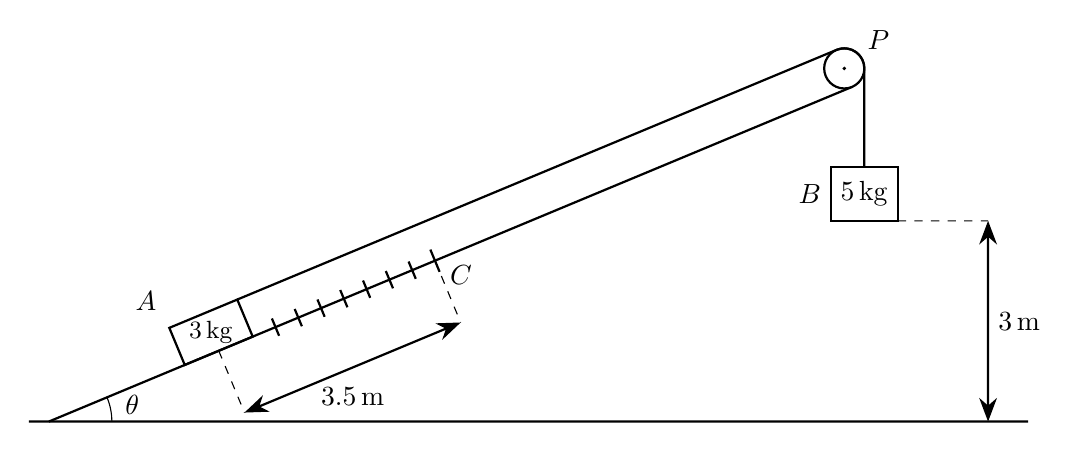
\begin{tikzpicture}[scale=0.85]
\def\run{12}
\def\rise{5}
\pgfmathsetmacro{\ang}{atan(\rise/\run)}
\pgfmathsetmacro{\slopeLen}{veclen(\run,\rise)}

\def\rad{0.30}
\def\bw{1.1}
\def\bh{0.60}
\def\hbw{1.0}
\def\hbh{0.8}

\def\AposFromBase{2.75}
\def\roughLen{3.5}
\def\Bclearance{3.0}
\pgfmathsetmacro{\halfBw}{0.5*\bw}

\coordinate (O) at (0,0);
\coordinate (X) at (2,0);
\coordinate (T) at (\run,\rise);
\pgfmathsetmacro{\afrac}{\AposFromBase/\slopeLen}
\coordinate (Apos) at ($(O)!\afrac!(T)$);
\coordinate (Aleft) at ($(Apos)+(\ang+180:\halfBw)$);
\coordinate (Afront) at ($(Apos)+(\ang:\halfBw)$);
\coordinate (C) at ($(Apos)+(\ang:\roughLen)$);

\coordinate (Pc) at ($(T)+(\ang+90:\rad)$);
\coordinate (Sleft) at ($(Pc)+(\ang+90:\rad)$);
\coordinate (Sright) at ($(Pc)+(0:\rad)$);

\pgfmathsetmacro{\drop}{\rise + \rad*cos(\ang) - (\Bclearance+\hbh)}
\coordinate (Btop) at ($(Sright)+(0,-\drop)$);
\coordinate (BbottomRight) at ($(Btop)+({\hbw/2},{-\hbh})$);
\coordinate (DimTop) at ($(BbottomRight)+(1.35,0)$);
\coordinate (DimBot) at ($(DimTop)+(0,-\Bclearance)$);

\draw[thick] (-0.3,0) -- ($(DimBot)+(0.6,0)$);
\draw[thick] (O) -- (T);

\pic[draw, "$\theta$", angle radius=8mm, angle eccentricity=1.35]
  {angle=X--O--T};

\foreach \i in {1,...,7} {
  \pgfmathsetmacro{\s}{\halfBw + \i*(\roughLen-\halfBw)/8}
  \coordinate (R\i) at ($(Apos)+(\ang:\s)$);
  \draw[thick] ($(R\i)+(\ang+90:0.14)$) -- ($(R\i)+(\ang-90:0.14)$);
}
\draw[thick] ($(C)+(\ang+90:0.18)$) -- ($(C)+(\ang-90:0.18)$);

\begin{scope}[shift={(Aleft)}, rotate=\ang]
  \draw[thick] (0,0) rectangle (\bw,\bh);
  \coordinate (Aattach) at (\bw,\bh);
  \coordinate (AupperLeft) at (0,\bh);
  \node[font=\small] at ({0.5*\bw},{0.5*\bh}) {$3\,\mathrm{kg}$};
\end{scope}

\fill[white] (Pc) circle (\rad);
\draw[thick] (Pc) circle (\rad);
\fill (Pc) circle (0.8pt);

\draw[thick]
  ($(Btop)+({-\hbw/2},0)$) rectangle ($(Btop)+({\hbw/2},{-\hbh})$);
\node at ($(Btop)+(0,{-0.5*\hbh})$) {$5\,\mathrm{kg}$};

\draw[thick] (Aattach) -- (Sleft);
\draw[thick] (Sleft) arc[start angle={\ang+90}, end angle=0, radius=\rad];
\draw[thick] (Sright) -- (Btop);

\node[above left] at ($(AupperLeft)+(\ang+90:0.12)$) {$A$};
\node[fill=white, inner sep=1pt, anchor=south east]
  at ($(C)+(\ang+90:-0.6)+(\ang:0.4)$) {$C$};
\node[anchor=west, inner sep=1pt]
  at ($(Pc)+(55:0.52)$) {$P$};
\node[left] at ($(Btop)+({-\hbw/2},{-0.5*\hbh})$) {$B$};


\coordinate (DimA) at ($(Apos)+(\ang-90:1.00)$);
\coordinate (DimC) at ($(C)+(\ang-90:1.00)$);
\draw[dashed] (Apos) -- (DimA);
\draw[dashed] (C) -- (DimC);
\draw[thick, {Stealth[length=3mm]}-{Stealth[length=3mm]}]
  (DimA) -- (DimC)
  node[midway, below=6pt, fill=white, inner sep=1pt] {$3.5\,\mathrm{m}$};

\draw[dashed] (BbottomRight) -- (DimTop);
\draw[thick, {Stealth[length=3mm]}-{Stealth[length=3mm]}]
  (DimBot) -- (DimTop)
  node[midway,right] {$3\,\mathrm{m}$};
\end{tikzpicture}
\end{figure}
\vspace*{10pt}

Two blocks, $A$ and $B$, of masses $3\,\mathrm{kg}$ and $5\,\mathrm{kg}$ respectively are attached to the ends of a light inextensible string. \\

Initially $A$ is held on a fixed plane. The plane is inclined to horizontal ground at an angle $\theta$, where $\tan\theta=\dfrac{5}{12}$. \\

The string passes over a small smooth light pulley $P$ that is fixed at the top of the plane. The part of the string from $A$ to $P$ is parallel to a line of greatest slope of the plane. \\

The section of the plane from the initial position of $A$ to a point $C$, $3.5\,\mathrm{m}$ up the plane, is rough. The section from $C$ to $P$ is smooth. \\

Block $B$ hangs freely below $P$ at a distance of $3\,\mathrm{m}$ above the ground, as shown in the diagram. The coefficient of friction between $A$ and the rough part of the plane is $\mu$. Block $A$ is released from rest with the string taut. \\

By modelling the blocks as particles, \\

\begin{enumerate}[label=\textbf{(\alph*)}]
  \item find the potential energy lost by the whole system as a result of $B$ falling $3\,\mathrm{m}$. \marks{3} \\
\end{enumerate}

Given that the speed of $B$ at the instant it hits the ground is $4.8\,\mathrm{m\,s^{-1}}$ and ignoring air resistance, \\

\begin{enumerate}[label=\textbf{(\alph*)}, resume]
  \item use the work-energy principle to find the value of $\mu$. \marks{6} \\
\end{enumerate}

After $B$ hits the ground, $A$ continues to move up the plane, passes $C$ and does not reach the pulley in the subsequent motion. \\

Block $A$ comes to instantaneous rest after moving a total distance of $(3.5+d)\,\mathrm{m}$ from its point of release. \\

Ignoring air resistance, \\

\begin{enumerate}[label=\textbf{(\alph*)}, resume]
  \item use the work-energy principle to find the value of $d$. \marks{4} \\
\end{enumerate}

\vspace*{10pt}

\begin{tcolorbox}[colback=white, colframe=scarlet, title={\textbf{Solution}}, breakable, grow to left by=6mm, grow to right by=10mm]
\begin{enumerate}[label=\textbf{(\alph*)}]
  \item From \(\tan\theta=\dfrac{5}{12}\), using a \(5\text{-}12\text{-}13\) triangle,
  \[
  \sin\theta=\frac{5}{13}
  \]

  If \(B\) falls \(3\,\mathrm{m}\), then \(A\) moves \(3\,\mathrm{m}\) up the plane, since the string is inextensible.

  So the vertical rise of \(A\) is
  \[
  3\sin\theta=3\times \frac{5}{13}=\frac{15}{13}\,\mathrm{m}
  \]

  Potential energy lost by \(B\):
  \[
  5g\times 3=15g
  \]

  Potential energy gained by \(A\):
  \[
  3g\times \frac{15}{13}=\frac{45g}{13}
  \]

  Therefore the net potential energy lost by the whole system is
  \begin{align*}
  15g-\frac{45g}{13}
  &=\frac{195g-45g}{13}\\
  &=\frac{150g}{13}
  \end{align*}

  With \(g=9.8\),
  \[
  \frac{150g}{13}=\frac{1470}{13}\,\mathrm{J}\approx 113\,\mathrm{J}
  \]

  So the potential energy lost is
  \[
  \frac{1470}{13}\,\mathrm{J}\approx 113\,\mathrm{J}
  \]

  \item Consider the motion from release until \(B\) hits the ground.

  For the whole two-block system, tension is internal, so the only non-conservative work is the work done by friction on \(A\).

  The gain in kinetic energy of the system is
  \begin{align*}
  \frac12(3+5)(4.8)^2
  &=\frac12(8)(4.8)^2\\
  &=92.16\,\mathrm{J}
  \end{align*}

  For block \(A\), perpendicular to the plane,
  \[
  R=3g\cos\theta=3g\times \frac{12}{13}=\frac{36g}{13}
  \]

  Hence the frictional force is
  \[
  \mu R=\mu\cdot \frac{36g}{13}
  \]

  Since \(A\) moves \(3\,\mathrm{m}\) along the rough plane, the work done against friction is
  \[
  \mu\cdot \frac{36g}{13}\cdot 3=\frac{108g\mu}{13}
  \]

  Now use the work-energy principle
  \[
  KE_0+GPE_0+\sum W = KE_1+GPE_1
  \]

  Here,
  \[
  KE_0=0,\qquad KE_1=92.16,\qquad \sum W=-\frac{108g\mu}{13}
  \]

  So
  \[
  0+GPE_0-\frac{108g\mu}{13}=92.16+GPE_1
  \]

  Rearranging,
  \[
  GPE_0-GPE_1=92.16+\frac{108g\mu}{13}
  \]

  From part (a),
  \[
  GPE_0-GPE_1=\frac{150g}{13}
  \]

  Hence
  \[
  \frac{150g}{13}=92.16+\frac{108g\mu}{13}
  \]

  Substituting \(g=9.8=\dfrac{49}{5}\),
  \[
  \frac{1470}{13}=\frac{2304}{25}+\frac{5292\mu}{65}
  \]

  So
  \begin{align*}
  \frac{5292\mu}{65}
  &=\frac{1470}{13}-\frac{2304}{25}\\
  &=\frac{36750-29952}{325}\\
  &=\frac{6798}{325}
  \end{align*}

  Therefore
  \begin{align*}
  \mu
  &=\frac{6798}{325}\cdot \frac{65}{5292}\\
  &=\frac{1133}{4410}\\
  &\approx 0.257
  \end{align*}

  So
  \[
  \mu=\frac{1133}{4410}\approx 0.257
  \]

  \item When \(B\) hits the ground, \(A\) is still moving at \(4.8\,\mathrm{m\,s^{-1}}\), and then continues up the plane alone.

  Since \(C\) is \(3.5\,\mathrm{m}\) from the start, and \(A\) has already moved \(3\,\mathrm{m}\), it travels a further
  \[
  3.5-3=0.5\,\mathrm{m}
  \]
  on the rough part, and then \(d\,\mathrm{m}\) on the smooth part.

  So after \(B\) hits the ground, the total distance moved by \(A\) is
  \[
  0.5+d
  \]

  Initial kinetic energy of \(A\):
  \begin{align*}
  \frac12\cdot 3\cdot (4.8)^2
  &=34.56\,\mathrm{J}
  \end{align*}

  Increase in gravitational potential energy of \(A\):
  \begin{align*}
  3g(0.5+d)\sin\theta
  &=3g(0.5+d)\cdot \frac{5}{13}\\
  &=\frac{147}{13}(0.5+d)
  \end{align*}

  Friction acts only over the remaining \(0.5\,\mathrm{m}\) of rough plane, so the work done against friction is
  \begin{align*}
  \mu R \times 0.5
  &=\mu\cdot \frac{36g}{13}\cdot 0.5\\
  &=\frac{18g\mu}{13}\\
  &=\frac{882\mu}{65}
  \end{align*}

  Now use the work-energy principle for block \(A\):
  \[
  KE_0+GPE_0+\sum W = KE_1+GPE_1
  \]

  Here,
  \[
  KE_0=34.56,\qquad KE_1=0,\qquad \sum W=-\frac{882\mu}{65}
  \]

  So
  \[
  34.56+GPE_0-\frac{882\mu}{65}=0+GPE_1
  \]

  Hence
  \[
  34.56=\left(GPE_1-GPE_0\right)+\frac{882\mu}{65}
  \]

  Therefore
  \[
  34.56=\frac{147}{13}(0.5+d)+\frac{882\mu}{65}
  \]

  Substitute \(\mu=\dfrac{1133}{4410}\):
  \[
  34.56=\frac{147}{13}(0.5+d)+\frac{882}{65}\cdot \frac{1133}{4410}
  \]

  \[
  34.56=\frac{147}{13}(0.5+d)+\frac{1133}{325}
  \]

  Write \(34.56=\dfrac{864}{25}\):
  \[
  \frac{864}{25}=\frac{147}{13}(0.5+d)+\frac{1133}{325}
  \]

  So
  \begin{align*}
  \frac{147}{13}(0.5+d)
  &=\frac{864}{25}-\frac{1133}{325}\\
  &=\frac{11232-1133}{325}\\
  &=\frac{10099}{325}
  \end{align*}

  Hence
  \begin{align*}
  0.5+d
  &=\frac{13}{147}\cdot \frac{10099}{325}\\
  &=\frac{10099}{3675}
  \end{align*}

  Therefore
  \begin{align*}
  d
  &=\frac{10099}{3675}-\frac12\\
  &=\frac{20198-3675}{7350}\\
  &=\frac{16523}{7350}\\
  &\approx 2.25
  \end{align*}

  So
  \[
  d=\frac{16523}{7350}\,\mathrm{m}\approx 2.25\,\mathrm{m}
  \]
\end{enumerate}
\end{tcolorbox}


\newpage

% ---- Question 5 ----
\questionitem
% [Source: _QBT___Solns__Work_Energy_Principle, Q5]


A crate, of mass $10\,\mathrm{kg}$, is pulled up a rough plane inclined at $15^\circ$ to the horizontal. \\

The crate is attached to a light string. The string lies in the vertical plane of greatest slope and is inclined at $20^\circ$ above the plane. \\

The tension in the string is $80$ newtons. \\

As the crate moves a distance of $x$ metres up the plane, its speed increases from $1.5\,\mathrm{m\,s^{-1}}$ to $4.5\,\mathrm{m\,s^{-1}}$. \\

The coefficient of friction between the crate and the plane is $0.3$. \\

\begin{enumerate}[label=\textbf{(\alph*)}]
  \item By using an energy method, find $x$. \marks{6} \\
  \item Describe how the model could be refined to obtain a more realistic value of $x$ and use an energy argument to explain whether this would increase or decrease the value of $x$. \marks{2} \\
\end{enumerate}

\vspace*{10pt}

\begin{tcolorbox}[colback=white, colframe=scarlet, title={\textbf{Solution}}, breakable, grow to left by=6mm, grow to right by=10mm]
\begin{enumerate}[label=\textbf{(\alph*)}]
  \item Let the normal reaction be $R$ N.

  First resolve perpendicular to the plane. There is no motion perpendicular to the plane, so the forces balance in that direction:
  \begin{align*}
  R + 80\sin 20^\circ &= 10g\cos 15^\circ \\
  R &= 98\cos 15^\circ - 80\sin 20^\circ
  \end{align*}
  Hence
  \begin{align*}
  R &\approx 98(0.9659) - 80(0.3420) \\
    &\approx 67.3\text{ N}
  \end{align*}

  So the friction force is
  \begin{align*}
  F &= \mu R \\
    &= 0.3R \\
    &\approx 0.3(67.3) \\
    &\approx 20.2\text{ N}
  \end{align*}

  Now apply the work-energy principle:
  \[
  \text{KE}_0 + \text{GPE}_0 + \sum W_k = \text{KE}_1 + \text{GPE}_1
  \]

  Take the initial position as zero gravitational potential energy.

  \begin{itemize}
    \item Initial kinetic energy:
    \[
    \text{KE}_0=\frac12 \times 10 \times 1.5^2
    \]
    \item Final kinetic energy:
    \[
    \text{KE}_1=\frac12 \times 10 \times 4.5^2
    \]
    \item Gain in height after moving $x$ m up a plane at $15^\circ$:
    \[
    x\sin 15^\circ
    \]
    so
    \[
    \text{GPE}_1=98x\sin 15^\circ
    \]
    \item Work done by the tension:
    \[
    80x\cos 20^\circ
    \]
    \item Work done against friction:
    \[
    -Fx=-0.3Rx
    \]
  \end{itemize}

  Substitute into the work-energy equation:
  \begin{align*}
  \frac12 \times 10 \times 1.5^2 + 80x\cos 20^\circ - 0.3Rx
  &= \frac12 \times 10 \times 4.5^2 + 98x\sin 15^\circ
  \end{align*}

  Rearranging,
  \begin{align*}
  80x\cos 20^\circ - 98x\sin 15^\circ - 0.3Rx
  &= \frac12 \times 10 \times (4.5^2-1.5^2) \\
  80x\cos 20^\circ - 98x\sin 15^\circ - 0.3(98\cos 15^\circ-80\sin 20^\circ)x
  &= 90
  \end{align*}

  Therefore
  \begin{align*}
  x &= \frac{90}{80\cos 20^\circ - 98\sin 15^\circ - 0.3(98\cos 15^\circ-80\sin 20^\circ)} \\
    &\approx 3.04
  \end{align*}

  Hence
  \[
  x \approx 3.04\text{ m}
  \]

  \item One refinement would be to include air resistance.

  Air resistance would do additional negative work on the crate. So in
  \[
  \text{KE}_0 + \text{GPE}_0 + \sum W_k = \text{KE}_1 + \text{GPE}_1
  \]
  the total work term $\sum W_k$ would be smaller for each metre travelled.

  Therefore, with the same tension of $80$ N, a greater distance is needed to produce the same increase in kinetic energy and gravitational potential energy.

  So a more realistic model including air resistance would make $x$ increase.
\end{enumerate}
\end{tcolorbox}


\newpage

% ---- Question 6 ----
\questionitem
% [Source: _QBT___Solns__Work_Energy_Principle, Q6]

\begin{figure}[H]
    \centering
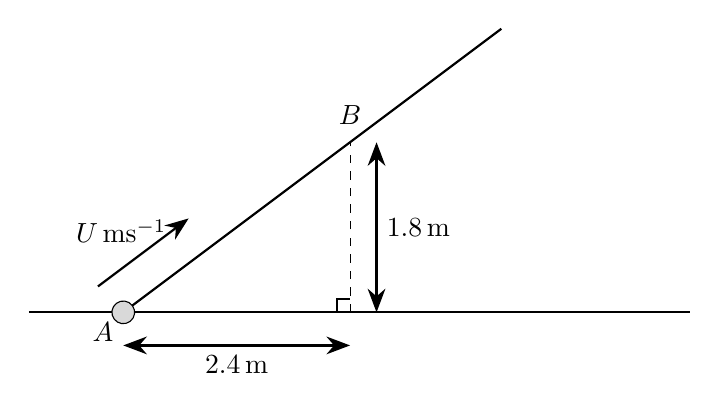
\begin{tikzpicture}[scale=1.2]
\def\horiz{2.4}
\def\rise{1.8}
\def\extra{2.0}
\def\groundleft{1.0}
\def\groundright{2.0}
\def\dimoff{0.35}
\def\voff{0.28}
\def\ra{0.14}
\def\particleRad{0.12}
\def\ustart{-0.05}
\def\uoffset{0.38}
\def\ulen{1.2}
\pgfmathsetmacro{\AB}{veclen(\horiz,\rise)}
\pgfmathsetmacro{\ang}{atan(\rise/\horiz)}
\pgfmathsetmacro{\mult}{1+\extra/\AB}
\pgfmathsetmacro{\groundend}{\horiz*\mult+\groundright}

\coordinate (A) at (0,0);
\coordinate (D) at (\horiz,0);
\coordinate (B) at (\horiz,\rise);
\coordinate (top) at ($(A)!\mult!(B)$);

\draw[thick, black] (-\groundleft,0) -- (\groundend,0);
\draw[thick, black] (A) -- (top);
\draw[dashed, black] (D) -- (B);

\draw[thick, black] ($(D)+(-\ra,0)$) -- ($(D)+(-\ra,\ra)$) -- ($(D)+(0,\ra)$);

\begin{scope}[shift={(A)}, rotate=\ang]
  \filldraw[fill=gray!30, draw=black] (0,0) circle (\particleRad);
  \draw[-{Stealth[length=3mm]}, thick, black] (\ustart,\uoffset) -- ++(\ulen,0)
    node[midway, above, xshift=-8pt] {$U\,\text{ms}^{-1}$};
\end{scope}

\draw[{Stealth[length=3mm]}-{Stealth[length=3mm]}, thick, black]
  ($(A)+(0,-\dimoff)$) -- ($(D)+(0,-\dimoff)$)
  node[midway, below] {$\horiz\,\text{m}$};

\draw[{Stealth[length=3mm]}-{Stealth[length=3mm]}, thick, black]
  ($(D)+(\voff,0)$) -- ($(B)+(\voff,0)$)
  node[midway, right] {$\rise\,\text{m}$};

\node[below left] at (A) {$A$};
\node[above, yshift=3pt] at (B) {$B$};
\end{tikzpicture}
\end{figure}


A rough loading ramp is fixed to horizontal ground. Point $A$ is the lower end of the ramp and point $B$ lies on the ramp above $A$, as shown in the diagram above. \\

The point vertically below $B$ is $2.4\,\text{m}$ horizontally from $A$, and $B$ is $1.8\,\text{m}$ above the ground. \\

A crate of mass $2.5\,\text{kg}$ is projected up the ramp from $A$ with speed $U\,\text{m s}^{-1}$ and first comes to instantaneous rest at $B$. \\

The coefficient of friction between the crate and the ramp is $\dfrac{1}{4}$. \\

The crate is modelled as a particle. \\

\begin{enumerate}[label=\textbf{(\alph*)}]
  \item Find the work done against friction as the crate moves from $A$ to $B$. \marks{3} \\
  \item Use the work-energy principle to find the value of $U$. \marks{4} \\
\end{enumerate}

After coming to instantaneous rest at $B$, the crate slides back down the ramp. \\

\begin{enumerate}[label=\textbf{(\alph*)}, resume]
  \item Use the work-energy principle to find the speed of the crate at the instant it returns to $A$. \marks{3} \\
\end{enumerate}

\vspace*{10pt}

\begin{tcolorbox}[colback=white, colframe=scarlet, title={\textbf{Solution}}, breakable, grow to left by=6mm, grow to right by=10mm]
\begin{enumerate}[label=\textbf{(\alph*)}]
  \item First find the length of the ramp.
  \[
  AB=\sqrt{2.4^2+1.8^2}=\sqrt{5.76+3.24}=\sqrt{9}=3\text{ m}
  \]

  Let the angle of the ramp to the horizontal be \(\theta\). Then
  \[
  \cos\theta=\frac{2.4}{3}=\frac45
  \]

  The normal reaction is
  \[
  R=mg\cos\theta=2.5g\times\frac45=2g
  \]

  So the friction force is
  \[
  F=\mu R=\frac14(2g)=\frac g2
  \]

  Hence the work done against friction from \(A\) to \(B\) is
  \[
  W=Fs=\frac g2\times 3=\frac{3g}{2}=14.7\text{ J}
  \]

  Therefore, the work done against friction is \(14.7\text{ J}\).

  \item Take \(A\) as the zero level for gravitational potential energy.

  From part (a), the work done against friction is \(14.7\text{ J}\), so the work done by friction is \(-14.7\text{ J}\).

  Using the work-energy principle
  \[
  \text{KE}_0+\text{GPE}_0+\sum W=\text{KE}_1+\text{GPE}_1
  \]

  for the motion from \(A\) to \(B\),
  \begin{align*}
  \frac12(2.5)U^2+0-14.7&=0+2.5g(1.8) \\
  1.25U^2-14.7&=44.1 \\
  1.25U^2&=58.8 \\
  U^2&=47.04
  \end{align*}

  Taking the positive root,
  \[
  U=\sqrt{47.04}=6.86\text{ m s}^{-1}
  \]

  Also,
  \[
  U=\frac{14\sqrt6}{5}\text{ m s}^{-1}
  \]

  Hence
  \[
  U=\frac{14\sqrt6}{5}\text{ m s}^{-1}\approx 6.86\text{ m s}^{-1}
  \]

  \item Let the speed of the crate when it returns to \(A\) be \(v\text{ m s}^{-1}\).

  The work done against friction is again \(14.7\text{ J}\), so the work done by friction is \(-14.7\text{ J}\).

  Using the work-energy principle
  \[
  \text{KE}_0+\text{GPE}_0+\sum W=\text{KE}_1+\text{GPE}_1
  \]

  for the motion from \(B\) to \(A\),
  \begin{align*}
  0+2.5g(1.8)-14.7&=\frac12(2.5)v^2+0 \\
  44.1-14.7&=1.25v^2 \\
  29.4&=1.25v^2 \\
  v^2&=23.52
  \end{align*}

  Taking the positive root,
  \[
  v=\sqrt{23.52}=4.85\text{ m s}^{-1}
  \]

  Also,
  \[
  v=\frac{14\sqrt3}{5}\text{ m s}^{-1}
  \]

  So the speed as it returns to \(A\) is
  \[
  \frac{14\sqrt3}{5}\text{ m s}^{-1}\approx 4.85\text{ m s}^{-1}
  \]
\end{enumerate}
\end{tcolorbox}


\newpage

% ---- Question 7 ----
\questionitem
% [Source: _QBT___Solns__Work_Energy_Principle, Q7]

\begin{figure}[H]
    \centering
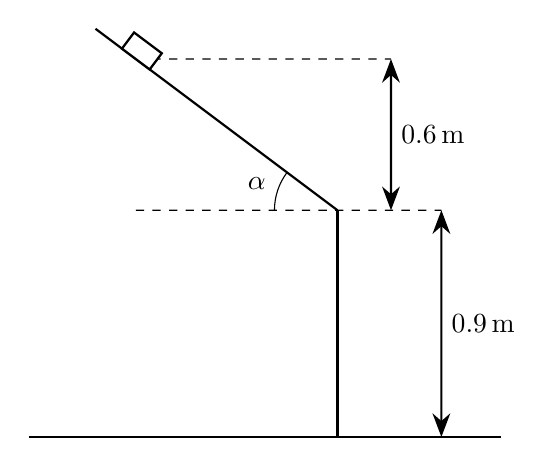
\begin{tikzpicture}[scale=0.8]
\pgfmathsetmacro{\ang}{asin(3/5)}
\pgfmathsetmacro{\roofang}{180-\ang}

\def\unit{4}
\pgfmathsetmacro{\eaveh}{0.9*\unit}
\pgfmathsetmacro{\rise}{0.6*\unit}
\pgfmathsetmacro{\roofdist}{\rise/sin(\ang)}
\pgfmathsetmacro{\rooflen}{\roofdist+0.8}

\def\boxw{0.55}
\def\boxh{0.32}
\def\dimsepA{0.85}
\def\dimsepB{1.65}

\coordinate (F) at (0,0);
\coordinate (E) at (0,\eaveh);
\coordinate (P) at ($(E)+(\roofang:\roofdist)$);
\coordinate (L) at ($(E)+(\roofang:\rooflen)$);
\coordinate (H) at (P|-E);

\coordinate (Vlo) at ($(E)+(\dimsepA,0)$);
\coordinate (Vhi) at ($(Vlo)+(0,\rise)$);
\coordinate (Wlo) at ($(F)+(\dimsepB,0)$);
\coordinate (Whi) at ($(Wlo)+(0,\eaveh)$);

\draw[thick] ($(F)+(-4.9,0)$) -- ($(F)+(2.6,0)$);
\draw[thick] (F) -- (E);
\draw[thick] (L) -- (E);

\draw[dashed] (P) -- (Vhi);
\draw[dashed] (H) -- (Whi);

\begin{scope}[shift={(P)}, rotate=\roofang]
  \draw[thick, fill=white] (-\boxw/2,0) rectangle (\boxw/2,-\boxh);
\end{scope}

\draw[{Stealth[length=3mm]}-{Stealth[length=3mm]}, thick] (Vlo) -- (Vhi)
  node[midway, right] {$0.6\,\mathrm{m}$};

\draw[{Stealth[length=3mm]}-{Stealth[length=3mm]}, thick] (Wlo) -- (Whi)
  node[midway, right] {$0.9\,\mathrm{m}$};

\path pic["$\alpha$", draw, angle radius=8mm, angle eccentricity=1.35]
  {angle=L--E--H};
\end{tikzpicture}
\end{figure}


A parcel of mass $m$ is held on a rough straight roof which is inclined at an angle $\alpha$ to the horizontal, where $\sin\alpha=\dfrac{3}{5}$. The parcel is released from rest at a point on the roof that is $0.6\,\mathrm{m}$ vertically above the eaves, as shown in the diagram above. The eaves are $0.9\,\mathrm{m}$ above the ground. The coefficient of friction between the parcel and the roof is $0.25$. \\

The parcel is modelled as a particle which, after leaving the roof, is assumed to move freely under gravity. \\

\begin{enumerate}[label=\textbf{(\alph*)}]
  \item Find, in terms of $m$ and $g$, the magnitude of the normal reaction on the parcel as it slides down the roof. \marks{2} \\
  \item Use the work-energy principle to find the speed of the parcel as it hits the ground. \marks{5} \\
\end{enumerate}

\vspace*{10pt}

\begin{tcolorbox}[colback=white, colframe=scarlet, title={\textbf{Solution}}, breakable, grow to left by=6mm, grow to right by=10mm]
\begin{enumerate}[label=\textbf{(\alph*)}]
  \item Resolving perpendicular to the roof, the parcel has no acceleration in this direction, so
  \[
  R = mg\cos\alpha
  \]
  
  Given \(\sin\alpha=\dfrac35\) and \(\alpha\) is acute,
  \[
  \cos\alpha=\frac45
  \]
  
  Hence
  \[
  R=mg\cdot\frac45=\frac{4mg}{5}
  \]
  
  So the magnitude of the normal reaction is \(\dfrac{4mg}{5}\).

  \item Let the distance travelled along the roof be \(s\) m.

  Since the vertical drop from the release point to the eaves is \(0.6\) m,
  \[
  s\sin\alpha=0.6
  \]
  so
  \[
  s=\frac{0.6}{3/5}=1
  \]
  
  Therefore the parcel slides \(1\) m along the roof.

  From part (a), the normal reaction is \(\dfrac{4mg}{5}\), so the friction force has magnitude
  \[
  F=\mu R=0.25\times \frac{4mg}{5}=\frac{mg}{5}
  \]
  
  Hence the work done by friction on the roof is
  \[
  -Fs=-\frac{mg}{5}\times 1=-\frac{mg}{5}
  \]
  
  The normal reaction does no work, since it is perpendicular to the motion. After the parcel leaves the roof, it moves freely under gravity, so there is no further friction.

  Take the ground as the zero level for GPE. The parcel starts at height
  \[
  0.6+0.9=1.5\text{ m}
  \]
  above the ground.

  Now use the work-energy principle
  \[
  \text{KE}_0+\text{GPE}_0+\sum W=\text{KE}_1+\text{GPE}_1
  \]
  
  Applying this from release to impact with the ground,
  \begin{align*}
  0 + mg(1.5) - \frac{mg}{5} &= \frac12 mv^2 + 0 \\
  \frac{3mg}{2}-\frac{mg}{5} &= \frac12 mv^2 \\
  \frac{15mg-2mg}{10} &= \frac12 mv^2 \\
  \frac{13mg}{10} &= \frac12 mv^2
  \end{align*}
  
  So
  \[
  v^2=\frac{13g}{5}
  \]
  and therefore
  \[
  v=\sqrt{\frac{13g}{5}}
  \]
  
  So the speed of the parcel as it hits the ground is \(\sqrt{\dfrac{13g}{5}}\ \mathrm{m\,s^{-1}}\).
\end{enumerate}
\end{tcolorbox}


\newpage

% ---- Question 8 ----
\questionitem
% [Source: _QBT___Solns__Work_Energy_Principle, Q8]

A rough plane is inclined to the horizontal at an angle $\theta$, where $\tan\theta=\dfrac{5}{12}$. \\

A particle $P$ of mass $m$ is at rest at a point $O$ on the plane. \\

The coefficient of friction between $P$ and the plane is $\dfrac{1}{4}$. \\

The particle is projected up the plane with speed $4\sqrt{ag}$. \\

The particle moves up a line of greatest slope of the plane, comes to instantaneous rest, and then slides back down to $O$. \\

\begin{enumerate}[label=\textbf{(\alph*)}]
  \item Show that the magnitude of the frictional force acting on $P$ is
  \[
  \dfrac{3mg}{13}
  \]
  \marks[-20pt]{3}
\end{enumerate}
Air resistance is assumed to be negligible. \\

Using the work-energy principle, \\

\begin{enumerate}[label=\textbf{(\alph*)}, resume]
  \item find the speed of $P$ when it returns to $O$. \marks{5} \\
\end{enumerate}

\vspace*{10pt}

\begin{tcolorbox}[colback=white, colframe=scarlet, title={\textbf{Solution}}, breakable, grow to left by=6mm, grow to right by=10mm]
\begin{enumerate}[label=\textbf{(\alph*)}]
  \item Since 
  \[
  \tan\theta=\frac{5}{12},
  \]
  we use the $5$-$12$-$13$ triangle, so
  \[
  \sin\theta=\frac{5}{13},\qquad \cos\theta=\frac{12}{13}.
  \]

  Perpendicular to the plane, the particle is in equilibrium, so the normal reaction is
  \[
  R=mg\cos\theta=mg\cdot \frac{12}{13}=\frac{12mg}{13}.
  \]

  The coefficient of friction is $\mu=\dfrac14$, so the magnitude of the frictional force is
  \[
  F=\mu R=\frac14\cdot \frac{12mg}{13}=\frac{3mg}{13}.
  \]

  Therefore, the magnitude of the frictional force is
  \[
  \frac{3mg}{13}.
  \]

  \item Let the particle travel a distance $s$ up the plane before coming to rest at the highest point $A$.

  From part (a), the frictional force has magnitude
  \[
  \frac{3mg}{13}.
  \]

  Also,
  \[
  \sin\theta=\frac{5}{13}.
  \]

  We use the work-energy principle in the form
  \[
  \text{KE}_0+\text{GPE}_0+\sum W=\text{KE}_1+\text{GPE}_1.
  \]

  Take the gravitational potential energy at $O$ to be $0$.

  \textit{Journey up the plane: from $O$ to $A$}

  Initial kinetic energy:
  \[
  \text{KE}_O=\frac12 m\left(4\sqrt{ag}\right)^2=\frac12 m(16ag)=8mag.
  \]

  Final kinetic energy at $A$:
  \[
  \text{KE}_A=0.
  \]

  Gain in gravitational potential energy:
  \[
  \text{GPE}_A=mg(s\sin\theta)=mg\left(s\cdot \frac{5}{13}\right)=\frac{5mgs}{13}.
  \]

  Work done by friction is negative, since friction opposes the motion:
  \[
  W_f=-\frac{3mg}{13}s.
  \]

  So
  \begin{align*}
  \text{KE}_O+\text{GPE}_O+\sum W&=\text{KE}_A+\text{GPE}_A \\
  8mag+0-\frac{3mgs}{13}&=0+\frac{5mgs}{13}.
  \end{align*}

  Hence
  \begin{align*}
  8mag&=\frac{8mgs}{13} \\
  s&=13a.
  \end{align*}

  \textit{Journey down the plane: from $A$ back to $O$}

  At $A$, the particle starts from rest, so
  \[
  \text{KE}_A=0.
  \]

  Its gravitational potential energy at $A$ is
  \[
  \text{GPE}_A=mg(s\sin\theta)=mg\left(13a\cdot \frac{5}{13}\right)=5mga.
  \]

  Friction again opposes the motion, so over distance $13a$ the work done by friction is
  \[
  W_f=-\frac{3mg}{13}(13a)=-3mga.
  \]

  Let the speed when it returns to $O$ be $v$. Then
  \[
  \text{KE}_O=\frac12 mv^2,\qquad \text{GPE}_O=0.
  \]

  Applying the work-energy principle:
  \begin{align*}
  \text{KE}_A+\text{GPE}_A+\sum W&=\text{KE}_O+\text{GPE}_O \\
  0+5mga-3mga&=\frac12 mv^2+0.
  \end{align*}

  So
  \begin{align*}
  2mga&=\frac12 mv^2 \\
  4ag&=v^2 \\
  v&=2\sqrt{ag}.
  \end{align*}

  Therefore, the speed when $P$ returns to $O$ is
  \[
  2\sqrt{ag}.
  \]
\end{enumerate}
\end{tcolorbox}


\newpage

% ---- Question 9 ----
\questionitem
% [Source: _QBT___Solns__Work_Energy_Principle, Q9]
\begin{figure}[H]
    \centering
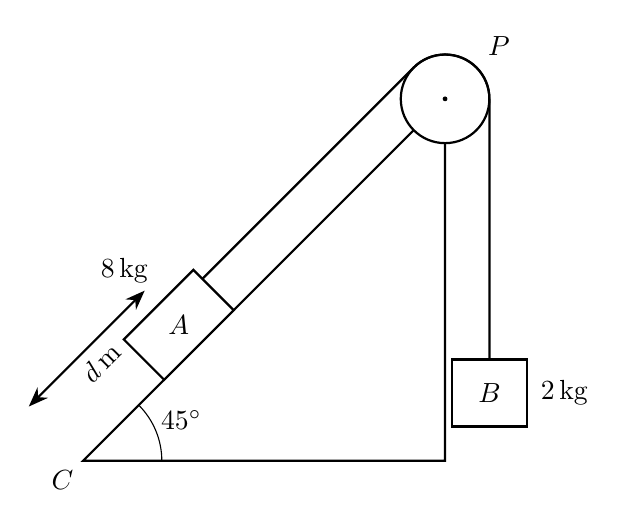
\begin{tikzpicture}[scale=1.25]
\def\ang{45}
\def\slopelen{5.2}
\def\pulrad{0.45}
\def\abw{1.0}
\def\abh{0.58}
\def\bbw{0.76}
\def\bbh{0.68}
\def\afrac{0.32}
\def\mdist{0.78}
\def\bdrop{2.65}
\pgfmathsetmacro{\run}{\slopelen*cos(\ang)}

\coordinate (C) at (0,0);
\coordinate (P) at (\ang:\slopelen);
\coordinate (R) at (\run,0);

\draw[thick] (C) -- (P) -- (R) -- cycle;

\pic["$45^\circ$", draw, angle radius=10mm, angle eccentricity=1.35]
  {angle=R--C--P};

\node[below left] at (C) {$C$};

\coordinate (Afoot) at ($(C)!\afrac!(P)$);
\begin{scope}[shift={(Afoot)}, rotate=\ang]
  \draw[thick, fill=white] (-\abw/2,0) rectangle (\abw/2,\abh);
  \coordinate (Acentre) at (0,\abh/2);
  \coordinate (Aattach) at (\abw/2,\pulrad);
  \node at (Acentre) {$A$};
\end{scope}
\node at ($(Acentre)+(\ang+90:0.78)$) {$8\,\mathrm{kg}$};

\coordinate (T1) at ($(P)+(\ang+90:\pulrad)$);
\coordinate (T2) at ($(P)+(0:\pulrad)$);

\draw[thick, fill=white] (P) circle (\pulrad);
\fill (P) circle (0.7pt);
\node[above right=1pt] at ($(P)+(45:\pulrad)$) {$P$};

\draw[thick] (Aattach) -- (T1);
\draw[thick] (T1) arc[start angle=\ang+90, end angle=0, radius=\pulrad];

\coordinate (Btop) at ($(T2)+(0,-\bdrop)$);
\coordinate (Bcentre) at ($(Btop)+(0,-\bbh/2)$);

\draw[thick, fill=white]
  ($(Btop)+(-\bbw/2,0)$) rectangle ($(Btop)+(\bbw/2,-\bbh)$);

\node at (Bcentre) {$B$};
\node[right=15pt] at (Bcentre) {$2\,\mathrm{kg}$};

\draw[thick] (T2) -- (Btop);

\coordinate (D0) at ($(C)+(\ang+90:\mdist)$);
\coordinate (D1) at ($(Afoot)+(\ang+90:\mdist)$);

\draw[{Stealth[length=2.5mm]}-{Stealth[length=2.5mm]}, thick]
  (D0) -- (D1) node[midway, sloped, below] {$d\,\mathrm{m}$};

\end{tikzpicture}
\end{figure}


One end of a rope is attached to a block $A$ of mass $8\,\mathrm{kg}$. The other end of the rope is attached to a second block $B$ of mass $2\,\mathrm{kg}$. Block $A$ is held at rest on a fixed rough ramp inclined at $45^\circ$ to the horizontal. The lower end of the ramp is $C$. The rope is taut and passes over a small smooth pulley $P$ which is fixed at the top of the ramp. The part of the rope from $A$ to $P$ is parallel to a line of greatest slope of the ramp. Block $A$ is initially $d\,\mathrm{m}$ from $C$, as shown in the diagram. \\

Block $B$ is more than $d\,\mathrm{m}$ below $P$. The blocks are released from rest and $A$ moves down the ramp towards $C$. \\

The coefficient of friction between $A$ and the ramp is $\dfrac{1}{4}$. \\

The blocks are modelled as particles, the rope is modelled as light and inextensible, and air resistance can be ignored. \\

\begin{enumerate}[label=\textbf{(\alph*)}]
  \item Determine, in terms of $g$ and $d$, the work done against friction as $A$ moves $d\,\mathrm{m}$ down the ramp. \marks{3} \\
  \item Given that the speed of $A$ immediately before it reaches $C$ is $2.1\,\mathrm{m\,s^{-1}}$, use the work-energy principle to determine the value of $d$. \marks{5} \\
  \item Suggest one improvement, apart from including air resistance, that could be made to the model to make it more realistic. \marks{1} \\
\end{enumerate}

\vspace*{10pt}

\begin{tcolorbox}[colback=white, colframe=scarlet, title={\textbf{Solution}}, breakable, grow to left by=6mm, grow to right by=10mm]
\begin{enumerate}[label=\textbf{(\alph*)}]
  \item Since $A$ moves down the ramp, friction acts up the ramp.

  The normal reaction on $A$ is
  \[
  R=8g\cos45^\circ=8g\cdot \frac{\sqrt2}{2}=4\sqrt2 g
  \]

  So the frictional force is
  \[
  F=\mu R=\frac14(4\sqrt2 g)=\sqrt2 g
  \]

  Hence the work done against friction as $A$ moves distance $d$ is
  \[
  W=Fd=(\sqrt2 g)(d)=\sqrt2 gd
  \]

  So the work done against friction is $\sqrt2 gd\ \mathrm{J}$.

  \item Consider the system consisting of both blocks $A$ and $B$.

  Since the rope is light and inextensible, both blocks have the same speed. Immediately before $A$ reaches $C$, this speed is $2.1\,\mathrm{m\,s^{-1}}$.

  Initially the system is at rest, so
  \[
  \mathrm{KE}_0=0
  \]

  The final kinetic energy is
  \[
  \mathrm{KE}_1=\frac12(8+2)(2.1)^2=22.05
  \]

  For block $A$, the vertical drop is $d\sin45^\circ$, so the loss in GPE of $A$ is
  \[
  8g(d\sin45^\circ)=8gd\cdot \frac{\sqrt2}{2}=4\sqrt2 gd
  \]

  For block $B$, it rises by $d$, so the gain in GPE of $B$ is
  \[
  2gd
  \]

  Therefore the overall loss in GPE of the system is
  \[
  \mathrm{GPE}_0-\mathrm{GPE}_1=4\sqrt2 gd-2gd
  \]

  From part (a), the work done against friction is $\sqrt2 gd$, so the work done by friction is
  \[
  -\sqrt2 gd
  \]

  Now use the work-energy principle
  \[
  \mathrm{KE}_0+\mathrm{GPE}_0+\sum W=\mathrm{KE}_1+\mathrm{GPE}_1
  \]

  Substituting in,
  \begin{align*}
  0+\mathrm{GPE}_0-\sqrt2 gd&=22.05+\mathrm{GPE}_1 \\
  \mathrm{GPE}_0-\mathrm{GPE}_1&=22.05+\sqrt2 gd
  \end{align*}

  But
  \[
  \mathrm{GPE}_0-\mathrm{GPE}_1=4\sqrt2 gd-2gd
  \]

  So
  \begin{align*}
  4\sqrt2 gd-2gd&=22.05+\sqrt2 gd \\
  3\sqrt2 gd-2gd&=22.05 \\
  (3\sqrt2-2)gd&=22.05
  \end{align*}

  Hence
  \[
  d=\frac{22.05}{g(3\sqrt2-2)}
  \]

  Using $g=9.8$,
  \begin{align*}
  d&=\frac{22.05}{9.8(3\sqrt2-2)} \\
  &=\frac{9}{4(3\sqrt2-2)} \\
  &=\frac{9(3\sqrt2+2)}{56} \\
  &\approx 1.00
  \end{align*}

  So
  \[
  d\approx 1.00\ \mathrm{m}
  \]

  \item One possible improvement is to model the pulley as not perfectly smooth, so friction at the pulley is taken into account.
\end{enumerate}
\end{tcolorbox}


\newpage

% ---- Question 10 ----
\questionitem
% [Source: _QBT___Solns__Work_Energy_Principle, Q10]

A small block of mass $0.5\,\mathrm{kg}$ is sliding down a rough slope which is inclined at $30^\circ$ to the horizontal. At the instant that its speed is $5\,\mathrm{m\,s^{-1}}$ directly down the slope, it is struck by a mallet. Immediately after the impact its speed is $12\,\mathrm{m\,s^{-1}}$ directly up the slope. \\

\begin{enumerate}[label=\textbf{(\alph*)}]
  \item Find the magnitude of the impulse exerted by the mallet on the block. \marks{2} \\
\end{enumerate}

After the impact, the block moves up the slope until it comes to instantaneous rest. It then slides back down the slope and passes through the point where it was struck with speed $4\,\mathrm{m\,s^{-1}}$. Assume that, whenever the block is moving, the resistance to its motion has constant magnitude $R\,\mathrm{N}$. \\

\begin{enumerate}[label=\textbf{(\alph*)}, resume]
  \item Use an energy method to determine the value of $R$. \marks{5} \\
\end{enumerate}

\vspace*{10pt}

\begin{tcolorbox}[colback=white, colframe=scarlet, title={\textbf{Solution}}, breakable, grow to left by=6mm, grow to right by=10mm]
\begin{enumerate}[label=\textbf{(\alph*)}]
  \item Take up the slope as positive. Then
  \[
  u=-5,\qquad v=12,\qquad m=0.5
  \]
  Impulse \(=\) change in momentum, so
  \[
  I=m(v-u)=0.5\bigl(12-(-5)\bigr)=0.5(17)=8.5
  \]
  Hence the magnitude of the impulse exerted by the mallet is \(8.5\,\mathrm{N\,s}\).

  \item Let the distance travelled up the slope before the block comes to rest be \(s\) m.

  Take the point where the block was struck as the zero of gravitational potential energy.

  For the upward motion, the initial speed is \(12\,\mathrm{m\,s^{-1}}\) and the final speed is \(0\).  
  The resistance and gravity both oppose the motion.

  Using the work-energy principle
  \[
  \mathrm{KE}_0+\mathrm{GPE}_0+\sum W=\mathrm{KE}_1+\mathrm{GPE}_1
  \]
  we have
  \begin{align*}
  \frac12(0.5)(12^2)+0+(-Rs) &= 0 + (0.5)gs\sin30^\circ \\
  36-Rs &= 0.25gs \\
  36 &= (0.25g+R)s
  \end{align*}

  Now consider the motion back down the slope from rest to the striking point, where the speed is \(4\,\mathrm{m\,s^{-1}}\).

  Again using
  \[
  \mathrm{KE}_0+\mathrm{GPE}_0+\sum W=\mathrm{KE}_1+\mathrm{GPE}_1
  \]
  gives
  \begin{align*}
  0+(0.5)gs\sin30^\circ+(-Rs) &= \frac12(0.5)(4^2)+0 \\
  0.25gs-Rs &= 4 \\
  (0.25g-R)s &= 4
  \end{align*}

  So
  \[
  (0.25g+R)s=36,\qquad (0.25g-R)s=4
  \]

  Adding the equations,
  \begin{align*}
  0.5gs &= 40 \\
  s &= \frac{80}{g}
  \end{align*}

  Substitute into \(36=(0.25g+R)s\)
  \begin{align*}
  36 &= \left(0.25g+R\right)\frac{80}{g} \\
  36 &= 20+\frac{80R}{g} \\
  16 &= \frac{80R}{g} \\
  R &= \frac{g}{5}
  \end{align*}

  With \(g=9.8\,\mathrm{m\,s^{-2}}\),
  \[
  R=\frac{9.8}{5}=1.96\,\mathrm{N}
  \]

  Therefore
  \[
  R=\frac{g}{5}\,\mathrm{N}=1.96\,\mathrm{N}
  \]
\end{enumerate}
\end{tcolorbox}


\end{enumerate}
\end{document}
